%%
% BIThesis 本科毕业设计论文模板 —— 使用 XeLaTeX 编译 The BIThesis Template for Undergraduate Thesis
% This file has no copyright assigned and is placed in the Public Domain.
%%

% 第一章节
\chapter{绪论}

\section{选题背景与意义}
% 这里插入一个参考文献，仅作参考


无人机（Unmanned Aerial Vehicle, UAV）作为飞行器与智能控制技术深度融合的代表性平台，近年来在军事侦察\cite{XDFJ202503001}、灾害救援\cite{WXYJ20250311005}、物流运输\cite{10138508}等领域展现出广阔的应用前景\cite{BIGO2023S2013, 20202696}。随着任务复杂度的不断提升，单一无人机在覆盖范围、系统鲁棒性及任务执行效率等方面的局限性日益凸显，促使研究重心逐步由单机控制向多无人机协同编队控制转变。由多个无人机组成的集群系统凭借高协同效率、强鲁棒性、功能多样性以及良好的可扩展性，已成为当前无人系统领域的研究热点\cite{张鹏飞2024无人机集群协同控制技术综述, 褚旭龙人工智能在无人机军事领域的应用发展研究:基于WOS核心数据库的文献计量分析}。尤其在战术对抗场景中，无人机集群能够有效实现协同侦察、分布式感知与协同打击等复杂任务，显著提升作战效能，如图\ref{无人机集群在军事作战场景中的应用示意图}所示\cite{fu2023icaus}。在此背景下，无人机集群技术的战略价值已获得全球主要国家的高度关注，并被相继纳入国家级科技与国防发展战略。美国《2017–2042无人系统综合路线图》明确提出构建“跨域协同杀伤力链”，着力推动空、天、网一体化的集群作战能力建设\cite{FHDD201808025, FHDD201905006}；俄罗斯于2023年发布《2030及2035年前无人航空发展战略》，旨在加速实现无人航空技术的自主可控与国产化替代\cite{HKDL202404004}；英国亦通过《机器人与自主系统战略2035》，加快智能无人系统在国防安全与公共事务领域的部署与应用\cite{UKSmartMachines2035}。这标志着无人机集群技术已从实验室阶段的学术探索，正式迈入关乎国家科技竞争力与战略安全的关键赛道。

\begin{figure}[H]
	\centering
	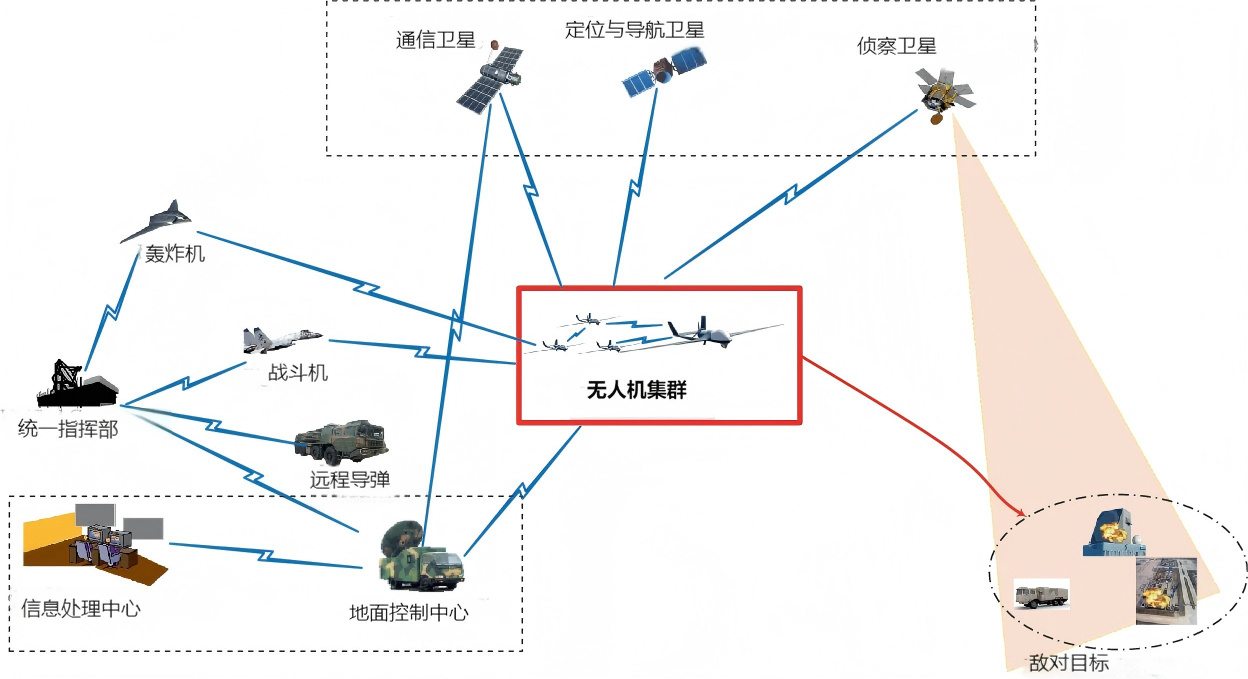
\includegraphics[width=0.8\linewidth]{images/1-1 - 副本}
	\caption[图片]{无人机集群在军事作战场景中的应用示意}
	\label{无人机集群在军事作战场景中的应用示意图}
	%\captionsetup{
	%	skip=5pt,        % 减小标题与图片的间距（默认较大）
	%	aboveskip=0pt,   % 图片上方与文本的间距
	%	belowskip=-10pt  % 图片下方与文本的间距
	%}
	%\vspace{-20pt}
\end{figure}

然而，尽管无人机集群在理想条件下已展现出强大潜力，其在真实复杂环境中的可靠运行仍面临严峻挑战。其中，状态信息获取受限是制约集群协同性能的核心瓶颈之一。在实际任务中，受限于传感器成本、功耗约束、通信带宽限制、电磁干扰或物理遮蔽等因素，集群中部分无人机往往无法获得完整的位置量测信息\cite{20202696}。例如，在城市峡谷、室内建筑、森林密林、地下空间或电磁干扰等——在这些全球导航卫星系统（Global Navigation Satellite System,GNSS）拒止环境中，GNSS信号易被遮挡、衰减甚至完全拒止，导致机载定位传感器失效或精度急剧下降，无人机难以获取高精度的三维绝对位置信息\cite{XXCN202401001, CSJX20250908001}。相较于传统集中式控制，无人机集群的分布式控制在复杂任务场景与非全维位置量测约束下展现出更为突出的适配性与性能优势。集中式控制虽具备控制精度高、实现逻辑简洁的特点，但高度依赖中心节点进行全局决策与任务分配，一旦核心节点失效或通信链路中断，整个集群将丧失协同能力，鲁棒性薄弱\cite{11207014}；且随着集群规模扩大，中心节点的通信带宽与计算负载呈指数级增长，难以满足大规模集群的扩展需求，尤其在GNSS拒止、电磁干扰等复杂环境中，中心节点与无人机间的信息交互易受干扰，进一步制约系统可靠性\cite{XXCN202401001}。

相较于传统的集中式控制架构，分布式控制通过去中心化设计，显著提升了无人机集群在复杂环境下的协同效能。其核心优势主要体现在以下四个方面：

\textbf{1）系统鲁棒性与容错能力：}在高对抗性或高动态任务环境中（如电子战干扰或城市巷战），通信链路极易受到遮蔽、干扰或人为切断，中心节点可能因物理损毁、通信中断或计算过载而突然失效\cite{JCGC202401005}。在此类场景下，传统集中式控制架构因其高度依赖单一决策中心进行全局状态感知与指令下发，一旦中心节点失联，整个集群将立即丧失协同能力，陷入无序飞行甚至碰撞瘫痪状态，严重制约系统在复杂战场中的生存性与任务连续性。相比之下，分布式控制摒弃了中心化决策范式，赋予每架无人机基于局部邻居状态信息自主更新行为的能力。这种“无中心、多备份”的机制使得系统具备天然的容错性：即使部分个体失效或局部通信链路中断，其余无人机仍可通过邻近交互维持编队结构与任务执行能力，有效避免单点故障引发全局崩溃。其根本原因在于，分布式一致性协议仅需通信拓扑保持弱连通（如联合连通图）即可保证状态收敛，无需全网信息可达，从而在不确定环境中实现高鲁棒协同\cite{1014083939.nh}。

\textbf{2）可扩展性与规模适应性：}在大规模集群任务（如百架以上广域协同侦察或分布式目标围捕）中，集中式控制架构面临严峻的可扩展性瓶颈。由于所有个体均需向中心节点上报状态并接收控制指令，通信负载高度集中于领航者节点，导致通信带宽迅速饱和；同时，中心节点需实时处理指数量级的状态数据并生成全局控制律，对计算资源提出极高要求，极易引发决策延迟甚至系统过载\cite{WXDG202301002}。这种“维度灾难”使得集中式方法难以支撑大规模集群任务的实时协同，严重限制了其在大规模作战场景中的应用潜力。而分布式架构通过将决策权下放至每个体，使每架无人机仅与有限数量的邻居交互，显著降低了单点通信压力与计算负担。系统整体通信与计算复杂度随集群规模近似线性增长，不仅避免了中心节点成为性能瓶颈，还使集群能够灵活适应规模的动态增减，无需重构全局控制逻辑。正因如此，分布式方法成为实现大规模协同任务的理想选择，有效解决了集中式架构在“大集群”场景下的性能瓶颈\cite{JCGC202401005}。

\textbf{3）复杂动态环境下的适应性：}真实任务场景常存在GNSS拒止、城市峡谷遮蔽或强电磁干扰等挑战，导致部分无人机无法获取完整的位置量测信息，仅能获得非全维状态（如缺失高度z轴、仅有水平面坐标，或仅能测量稀疏相对距离。传统集中式控制依赖中心节点融合全局高精度状态以生成统一指令，一旦输入信息残缺，极易因控制律失配而引发队形发散甚至碰撞。相比之下，分布式控制允许个体仅利用邻近无人机的相对量测实现渐近一致运动。即便部分维度信息缺失，只要通信拓扑满足基本连通性条件，集群仍可通过自组织协同维持期望队形，显著提升在状态受限环境中的鲁棒性与任务可靠性\cite{1014083939.nh}。

\textbf{4）异构平台的任务适应能力：}未来无人机集群将呈现高度异构化特征，系统中可能同时包含四旋翼、固定翼、通信支撑型及作战侦察型等多种类型无人机，其动力学模型、执行能力与传感器配置差异显著\cite{JSFY202504007}。分布式控制架构可通过分层协同机制实现异构无人机间的高效协作。具体而言，无人机集群系统上层利用任务分配算法（如合同网拍卖机制）将全局目标划分为多个子任务\cite{XTYD202111033}，或利用异构目标任务约束实现多异构无人机任务分配的建模\cite{QBZH202506006}，而下层各无人机根据自身能力特性（如机动性能、载重能力、载荷类型等）自主完成协同规划与控制。以城市反恐任务为例，固定翼无人机巡飞扫描敌情，而多旋翼无人机凭借其优良的机动性能与悬停能力承担抵近目标建筑精细化观测任务。二者实时共享数据，固定翼传外围警戒信息，四旋翼补盲区细节，助力构建实时战场态势图。这种分工模式整合不同异构平台的优势，提升了系统整体的任务完成效率，降低风险，也增强了对任务的适应能力\cite{YCYK202404001}。


因此，面向非全维位置量测约束，研究兼具稳定性、鲁棒性与实用性的分布式编队控制方法，不仅是突破当前集群协同性能瓶颈的关键路径，更是推动无人机集群从“理想实验室环境”走向“真实复杂战场/任务场景”的核心技术支撑。本课题正是在此背景下提出，强调可实现性与工程落地，通过仿真平台完成方案设计与验证，旨在为保障无人机集群在复杂环境下的任务可靠性与安全性具有重要的理论意义与工程价值。

\section{国内外研究现状}
% 这里插入一个参考文献，仅作参考

\subsection{国内外无人机集群项目进展}
近年来，随着人工智能、自主控制与通信网络等技术的快速发展，无人机集群系统已从理论探索逐步迈向工程化部署。全球主要国家纷纷启动国家级无人机集群项目，旨在提升其在复杂场景中的协同能力，尤其是在军事战术场景中的能力。本小节通过各国典型的战略集群项目与军事场景应用案例，梳理无人机集群相关技术的研究现状、发展路线及未来挑战，旨在揭示无人机集群的研究内核与发展方向。

美国作为世界上最早开展无人机集群相关研究工作的国家，其在无人机集群作战系统的概念、项目研究、作战装备、关键技术等方面，一直处于世界领先地位\cite{WRXT202409001016}。美国军方将无人机集群视为实现“第三次抵止战略”的关键一环，其发展路径具有顶层设计清晰、项目牵引明确、虚实结合紧密的特点\cite{zha2024smart}。以国防高级研究计划局（DARPA）为主导，美国启动了一系列具有里程碑意义的项目\cite{JSWN202005010}。
其中，“进攻性蜂群使能战术”（OFFSET）项目聚焦于城市巷战这一高复杂度场景，旨在实现250个以上异构无人平台协作，在通信传感受限的城市环境中6小时内完成8个街区任务。该项目围绕群体智能、平台自主、人机协同三大关键技术攻关，通过顶层设计、AI 赋能、仿真验证加速实战转化，为未来无人集群重塑城市作战模式。该项目已完成五次技术冲刺，于2021年底圆满完成最后一次现场实验，见图1-2中的子图(a)，通过无人蜂群重塑城市作战规则，使美军小单位部队具备“以少胜多、以低耗胜高耗”的核心能力\cite{KJPL202008007}。
此外，“拒止环境协同作战”（CODE）项目针对高对抗、通信受限战场下集中式控制易失效的问题，重点发展了面向无人机集群的分布式协同控制架构。该架构摒弃对中央节点的强依赖，转而赋予各平台基于局部感知与有限通信的自主决策能力，并通过任务预案机制实现去中心化的任务分配与行为协调。关键技术突破在于构建了一种支持多层级干预的分布式控制框架：在通信正常时，操作员可进行高层意图引导；一旦链路中断或遭遇突发威胁，集群能依据预设规则与在线推演，在无中心调度的情况下自主重构任务、规避风险并维持编队协同。飞行验证表明，该分布式控制方法显著提升了系统的鲁棒性与任务持续性，同时大幅降低操作员认知负荷，为复杂对抗环境下大规模无人机集群的自主、弹性、协同控制提供了核心技术路径\cite{FHDD201905005}。
为应对战场前沿对快速响应、多平台部署蜂群能力的迫切需求，美国海军研究实验室启动“低成本无人机集群技术”（LOCUST）项目，发展“郊狼”无人机系统，旨在解决传统无人机发射平台适配性差、难以在拒止环境中持续作战等瓶颈。其关键技术突破在于采用管式折叠设计与高速连续发射机制，支持在不同平台下30秒内密集齐射数十架无人机，并通过自组网与协同飞控算法实现发射后自动展开、编队与任务执行。自2016年完成30架集群飞行试验以来，“郊狼”已演进为兼具反无人机拦截与进攻性蜂群打击能力的多用途平台，并被整合至陆军M-LIDS和海军“宙斯盾”系统,见图1-2中的子图(b)。该项目显著提升了美军在复杂电磁环境下的分布式感知、电子战与饱和攻击能力，实现了低成本蜂群从概念验证向实战部署的关键跨越\cite{JCGC202208001,BGZD202503021}。
这些项目共同构成了美国无人机集群技术从基础算法、平台硬件到战术战法的完整研发生态，其最终目标是将集群智能深度融入未来“马赛克战”等高端作战体系，以形成非对称的战略优势。

\begin{figure}[H]
	\centering
	\subfloat[OFFSET项目实验]{
		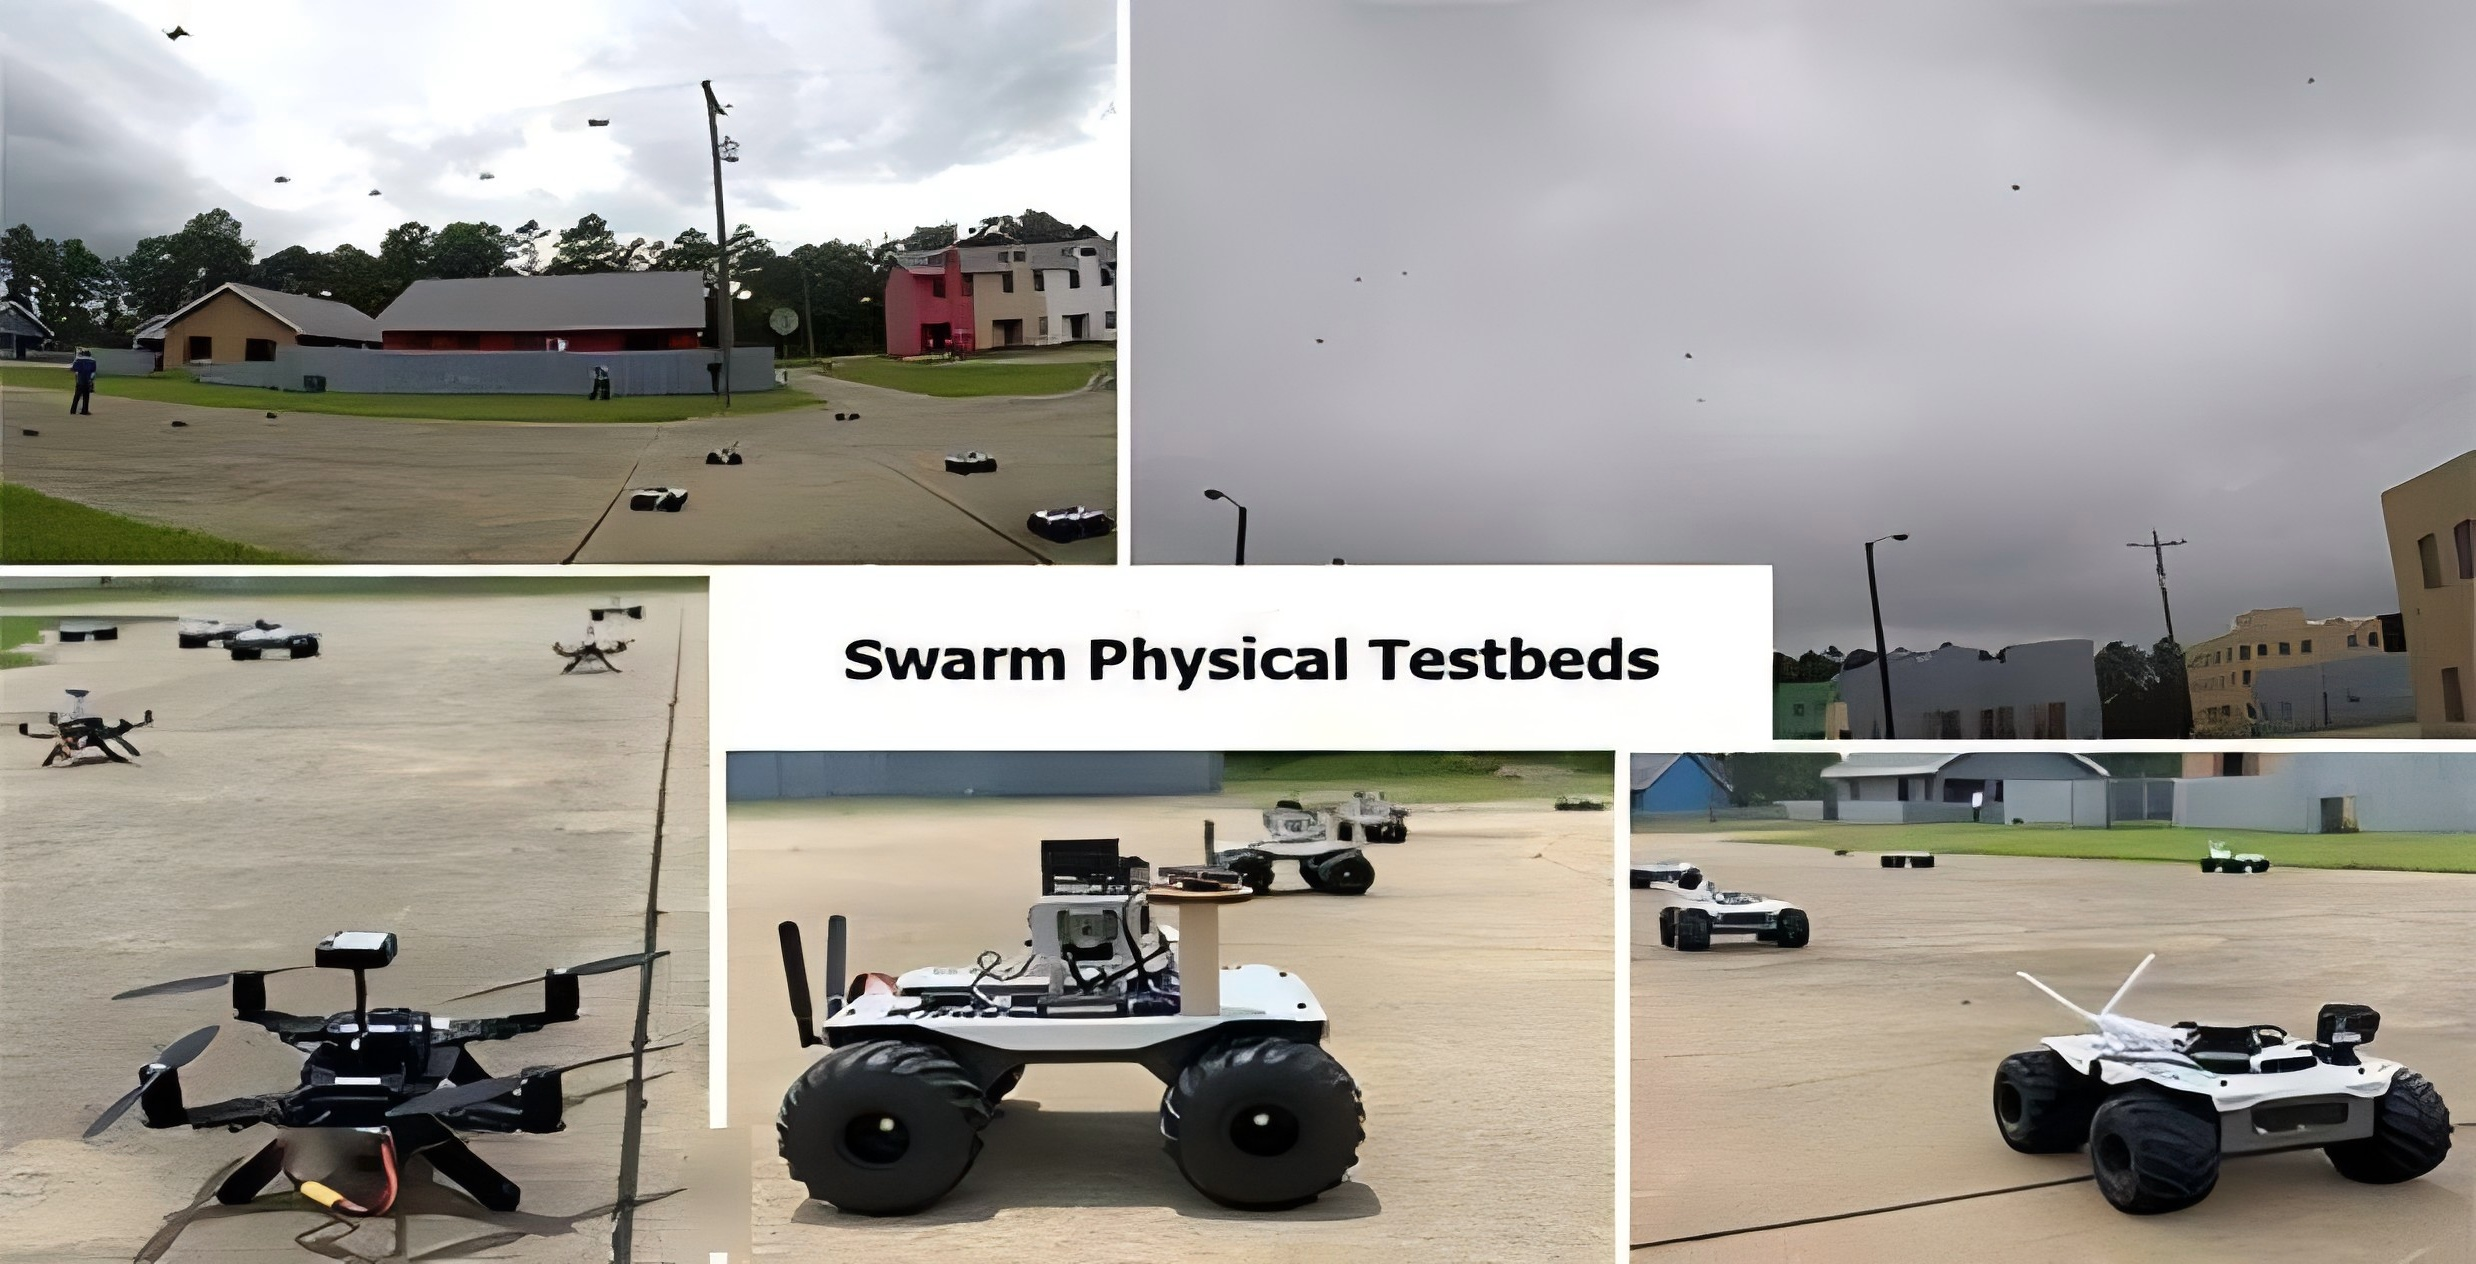
\includegraphics[height=4cm, keepaspectratio]{images/1-2-a}
	}
	\subfloat[“郊狼”多用途平台]{
		\includegraphics[height=4cm, keepaspectratio]{images/1-2-b}
	}
	\caption{美国无人机集群相关的典型军事项目}
	\label{1-2}
	% \vspace{-20pt}
\end{figure}

在俄乌冲突中，俄罗斯将“天竺葵-2”自杀式无人机作为实施战略消耗与纵深打击的关键手段，频繁用于对乌克兰能源设施、军工企业及军事基地的大规模夜间空袭。其核心战法是通过高密度集群发射形成饱和攻击，迫使乌方以成本高昂的防空导弹拦截极低成本的无人机，从而在效费比上取得显著优势。为提升突防能力，“天竺葵-2”不断优化飞行策略，从早期超低空掠地飞行转向高空突防，并强化导航系统的抗干扰性能，采用多天线相控阵模块和复合制导技术以应对日益增强的电子对抗环境。同时，其战斗部持续升级，增强对加固目标的毁伤效果。未来，“天竺葵”系列正向更高自主性和多功能化演进，如“天竺葵-3”已尝试换装喷气发动机以提高速度，并探索挂载空空导弹用于反制拦截战机，显示出向侦察、诱骗、打击一体化蜂群体系发展的趋势\cite{thedrive_perdix_shahed,TKZJ202516014}。
与“天竺葵”侧重战略纵深打击不同，俄罗斯国产的“柳叶刀”巡飞弹则聚焦于前线战术精确猎杀，在战场上承担反炮兵、反装甲及防空压制等任务。它凭借光电与红外复合导引头以及初步集成的AI图像识别能力，可在复杂环境中自主识别并锁定高价值移动或静止目标。其设计强调隐蔽性与快速部署能力，采用折叠翼结构和电动推进系统，噪音低、雷达特征小，适合在敌方前沿区域隐蔽行动。近年来，“柳叶刀”的制导精度与任务灵活性不断提升，支持人在回路控制与有限自主模式切换，并开始尝试多机协同作战，例如通过连续波次攻击突破物理防护网。俄军还将其与侦察无人机配合作战，构建简易的“察打一体”闭环。尽管受限于微电子供应链，俄方仍通过民用器件替代和模块化设计维持产能与迭代速度。整体来看，“柳叶刀”正朝着小型化、智能化和集群协同方向稳步发展，成为俄军战术层面不可或缺的精确打击节点\cite{TKZJ202401009,janes_lancet_ai}。

\begin{figure}[H]
	\centering
	\subfloat[“天竺葵-2”自杀式无人机]{
		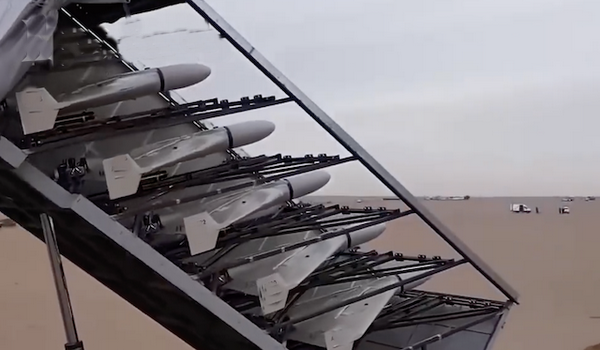
\includegraphics[height=4cm, keepaspectratio]{images/1-3-a}
	}
	\subfloat[“柳叶刀”巡飞弹]{
		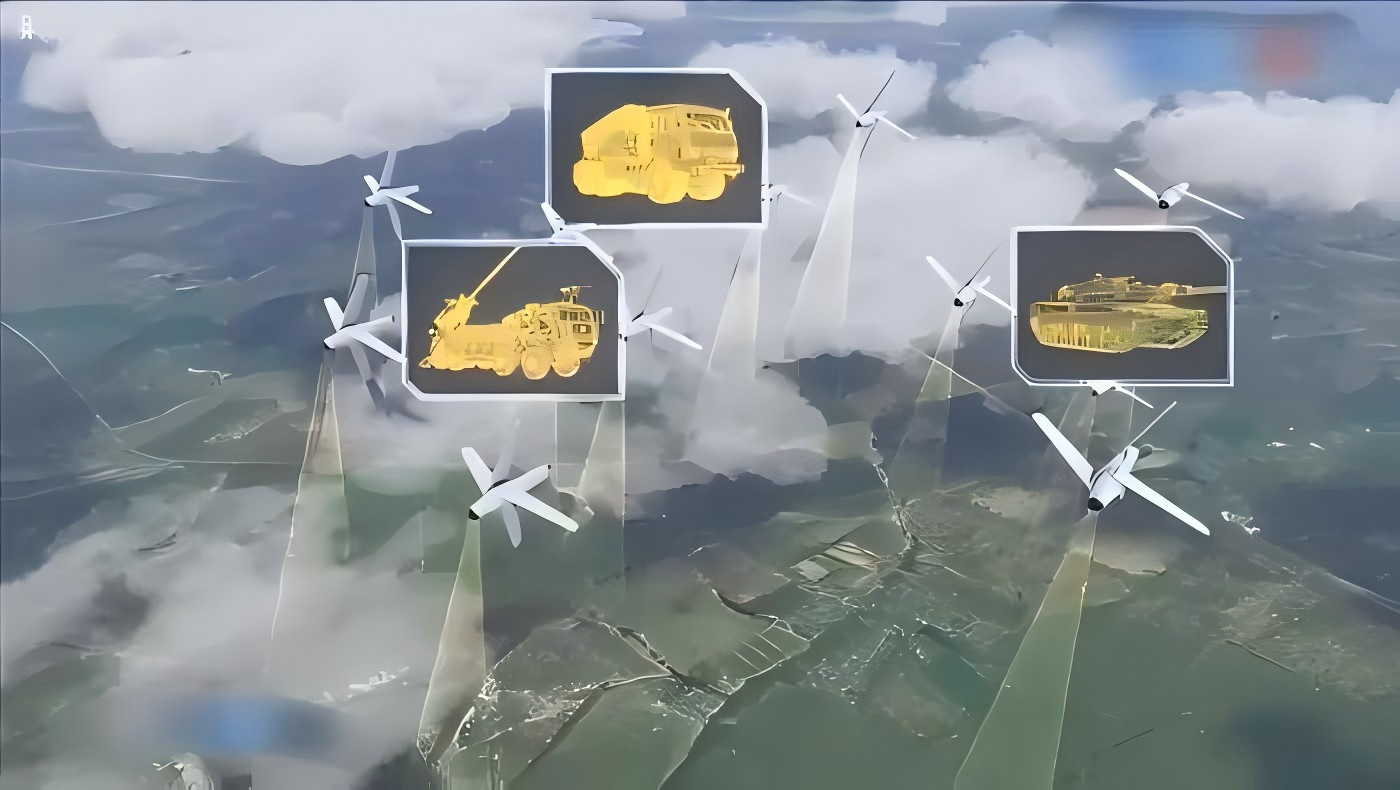
\includegraphics[height=4cm, keepaspectratio]{images/1-3-b}
	}
	\caption{俄罗斯无人机集群}
	\label{1-3}
	% \vspace{-20pt}
\end{figure}

除了上述研发项目之外，无人机集群已大量应用于军事对抗场景中。俄乌冲突中，俄军对无人机蜂群战术的运用，给乌克兰军队带来了前所未有的压力。俄军依托大量低成本的“天竺葵-2”自杀式无人机，频繁实施蜂群式饱和攻击，对乌克兰能源设施、军事基地等关键目标构成持续威胁。其优势在于数量庞大、成本低廉、低空突防能力强，能从多方向同时进袭，有效压缩乌军反应时间。面对此类集群攻击，乌军传统防空体系暴露出严重短板：高射炮火力覆盖有限，难以应对多点突防；昂贵的防空导弹拦截效费比极低，资源迅速枯竭；而城市地形与地球曲率进一步限制了雷达对低空目标的探测能力。尽管乌方引入“猎豹”高炮、“爱国者”等先进系统，并尝试轻武器拦截，仍难以构建高效、可持续的反蜂群防御体系，凸显了传统防空模式在应对大规模、低成本无人机集群时的根本性局限\cite{sohu_swarm_2025}。

从美国“进攻性蜂群使能战术”项目到俄乌冲突中无人机蜂群战术的实战应用，无人机集群展现了强大的应用前景。无论技术路径存在何种差异，其能力演进均高度依赖复杂环境下鲁棒、高效的编队控制能力。
\subsection{编队控制研究进展}
无人机集群编队控制旨在使多架无人机在协同飞行过程中维持预设几何构型并完成共同任务。相关技术发展路径因传感器性能、通信拓扑和控制逻辑的差异呈现多样性，见表\ref{无人机集群编队控制方法对比表}。根据控制架构与信息交互方式的不同，现有编队控制方法主要可分为领航-跟随法、基于势场的方法、基于行为的方法以及一致性理论的控制方法等四大类。这些方法在量测依赖、控制精度、鲁棒性及可扩展性等方面各具特点，适用于不同任务场景。

\begin{table}[H]
	\centering
	\caption{无人机集群编队控制方法对比}
	% \makebox[\linewidth]{} 让表格撑满页宽，@{}清除左右边距，c{宽度}让列居中且均分宽度
	\makebox[\linewidth][c]{
		\begin{tabular}{@{}ccccc@{}} % 全部列改为居中对齐（c），@{}清除左右边距
			\toprule  % 顶部粗线
			控制方法 & 所需量测条件 & 控制变量 & 网络拓扑 \\
			\midrule  % 中部细线
			领航-跟随法 & 相对位置 & 相对位置 & 有向星型图 \\
			基于势场的方法 & 全局位置 & 全局位置 & 集中式广播拓扑 \\
			基于行为的方法 & 相对位置/速度 & 相对位置/速度 & 近邻交互无向图 \\
			一致性理论的控制方法 & 全局状态 & 全局状态 & 连通有向/无向图 \\
			\bottomrule % 底部粗线
		\end{tabular}
	}
	\label{无人机集群编队控制方法对比表}
\end{table}

领航-跟随法是多智能体系统编队控制领域中的重要范式，其核心思想基于角色分工与层级关系。该方法将无人机集群中的个体明确划分为领航者与跟随者两类角色，如图\ref{领航-跟随法}所示。其基本思想是集群内领航者自主飞行，跟随者接收领导者的控制指令调整自身运动参数，以维持在编队中相对位置，同时反馈自身信息给领航者集中处理，从而实现编队控制。针对大规模固定翼无人机集群在复杂任务中队形适应性差、控制维度高、协同效率低的问题。文献\parencite{1022813032.nh}创新性地将仿射编队控制与分层架构结合，通过控制少量关键节点即可完成大规模固定翼无人机集群的仿射变换，显著提升了编队机动性与可扩展性。文献\parencite{XDYX20250820001}针对有人-无人机编队中传统领航-跟随法在有人机机动时易导致队形破坏和碰撞的问题，提出一种融合虚拟弹簧避障机制，并引入对有人机飞行姿态的跟踪算法，使无人机能同步维持期望相对位置与姿态，从而在机动过程中保持队形稳定并避免内外部碰撞。文献\parencite{BJHK202407029}针对多领导者无人机集群中领导者无法形成时变编队、且缺乏明确编队中心描述的问题，提出一种领导-跟随双层编队跟踪控制方法，设计含领导者编队项与跟随者跟踪项的分布式协议，给出编队中心显式表达式及跟踪充分条件，并通过Riccati方程求解控制器增益，实现了领导者与跟随者各自形成时变编队且整体协同跟踪。文献\parencite{ANGHELUTA202573}聚焦于领航-跟随者层级架构，结合图刚性理论与Lyapunov稳定性分析，为单/双积分器动力学模型设计了抗扰动的分布式距离约束控制律，并在DJI Tello四旋翼平台上完成了实验验证，有效保障了该控制方法编队的形状保持与运动一致性。

\begin{figure}[H]
	\centering
	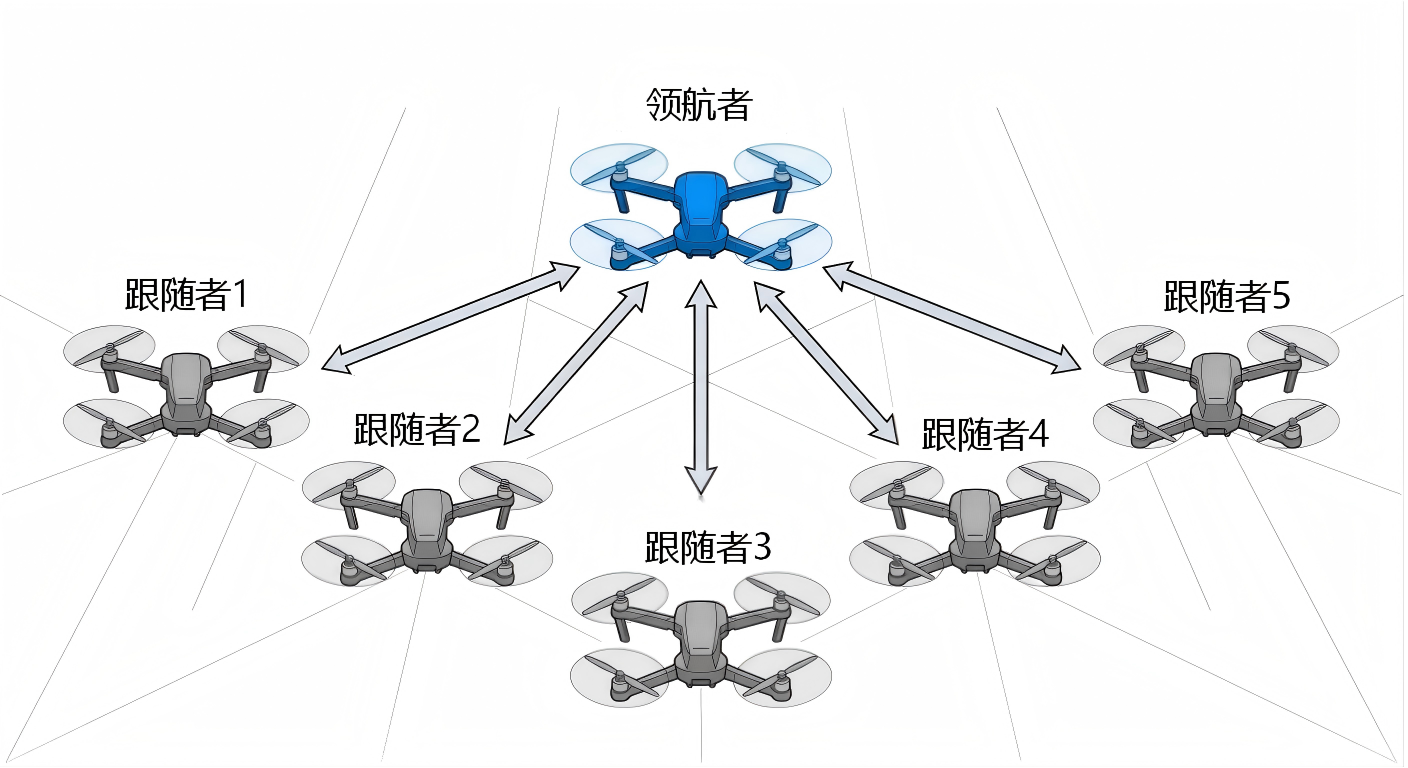
\includegraphics[height=5cm, keepaspectratio]{images/1-4}
	\caption{领航-跟随法}
	\label{领航-跟随法}
	%\vspace{-10pt}
\end{figure}

基于势场的编队控制方法借鉴了物理学中势场概念，为集群内无人机设计势场函数，在感知范围内，依据无人机之间相邻距离设置排斥区、保持区、吸引区，排斥区内相邻无人机会受斥力拉大距离，保持区内无人机控制参数保持不变，吸引区内相邻无人机受引力缩小距离，通过势场力使得每架无人机收敛到期望位置，从而保持编队队形，如图\ref{基于势场的编队控制方法}所示。文献\parencite{DZGS202504038}针对传统人工势场法无法维持固定队形的问题，提出将虚拟结构与人工势场融合——每架无人机受其对应虚拟结构点的引力和邻机斥力共同作用，在保持预设几何构型的同时实现避碰，提升了编队稳定性与安全性。文献\parencite{FHLX201903008}针对集群在目标跟踪中队形易散、避障能力弱的问题，设计双层虚拟质点，通过分层势场引导个体先聚集成队、再整体跟踪目标，实现了队形保持、协同避障与轨迹跟踪的一体化控制。此外，针对基于人工势场的群体聚集模型仅适用于理想“运动学”个体、难以应用于具有复杂动力学和不确定性的实际工程系统的问题，文献\parencite{1549948}提出一种结合人工势场与滑模控制的实现方法。通过滑模控制器驱动具有不确定动力学的无人机跟踪势场生成的理想运动指令，从而在存在扰动和模型不确定性的情况下，仍能鲁棒实现群体聚集与队形控制，为理论模型向工程应用转化提供了有效途径。文献\parencite{XAJT201811017}针对传统人工势场法在无人机编队避障中易陷入局部极小值的问题，提出一种三维复合矢量人工势场法，通过构建平面的旋转斥力场，打破共线平衡，引导编队选择最优路径绕障，并在避障后快速重组三角形队形，有效提升了避障成功率与路径优化能力，克服了传统势场法的局部极小问题。

\begin{figure}[H]
	\centering
	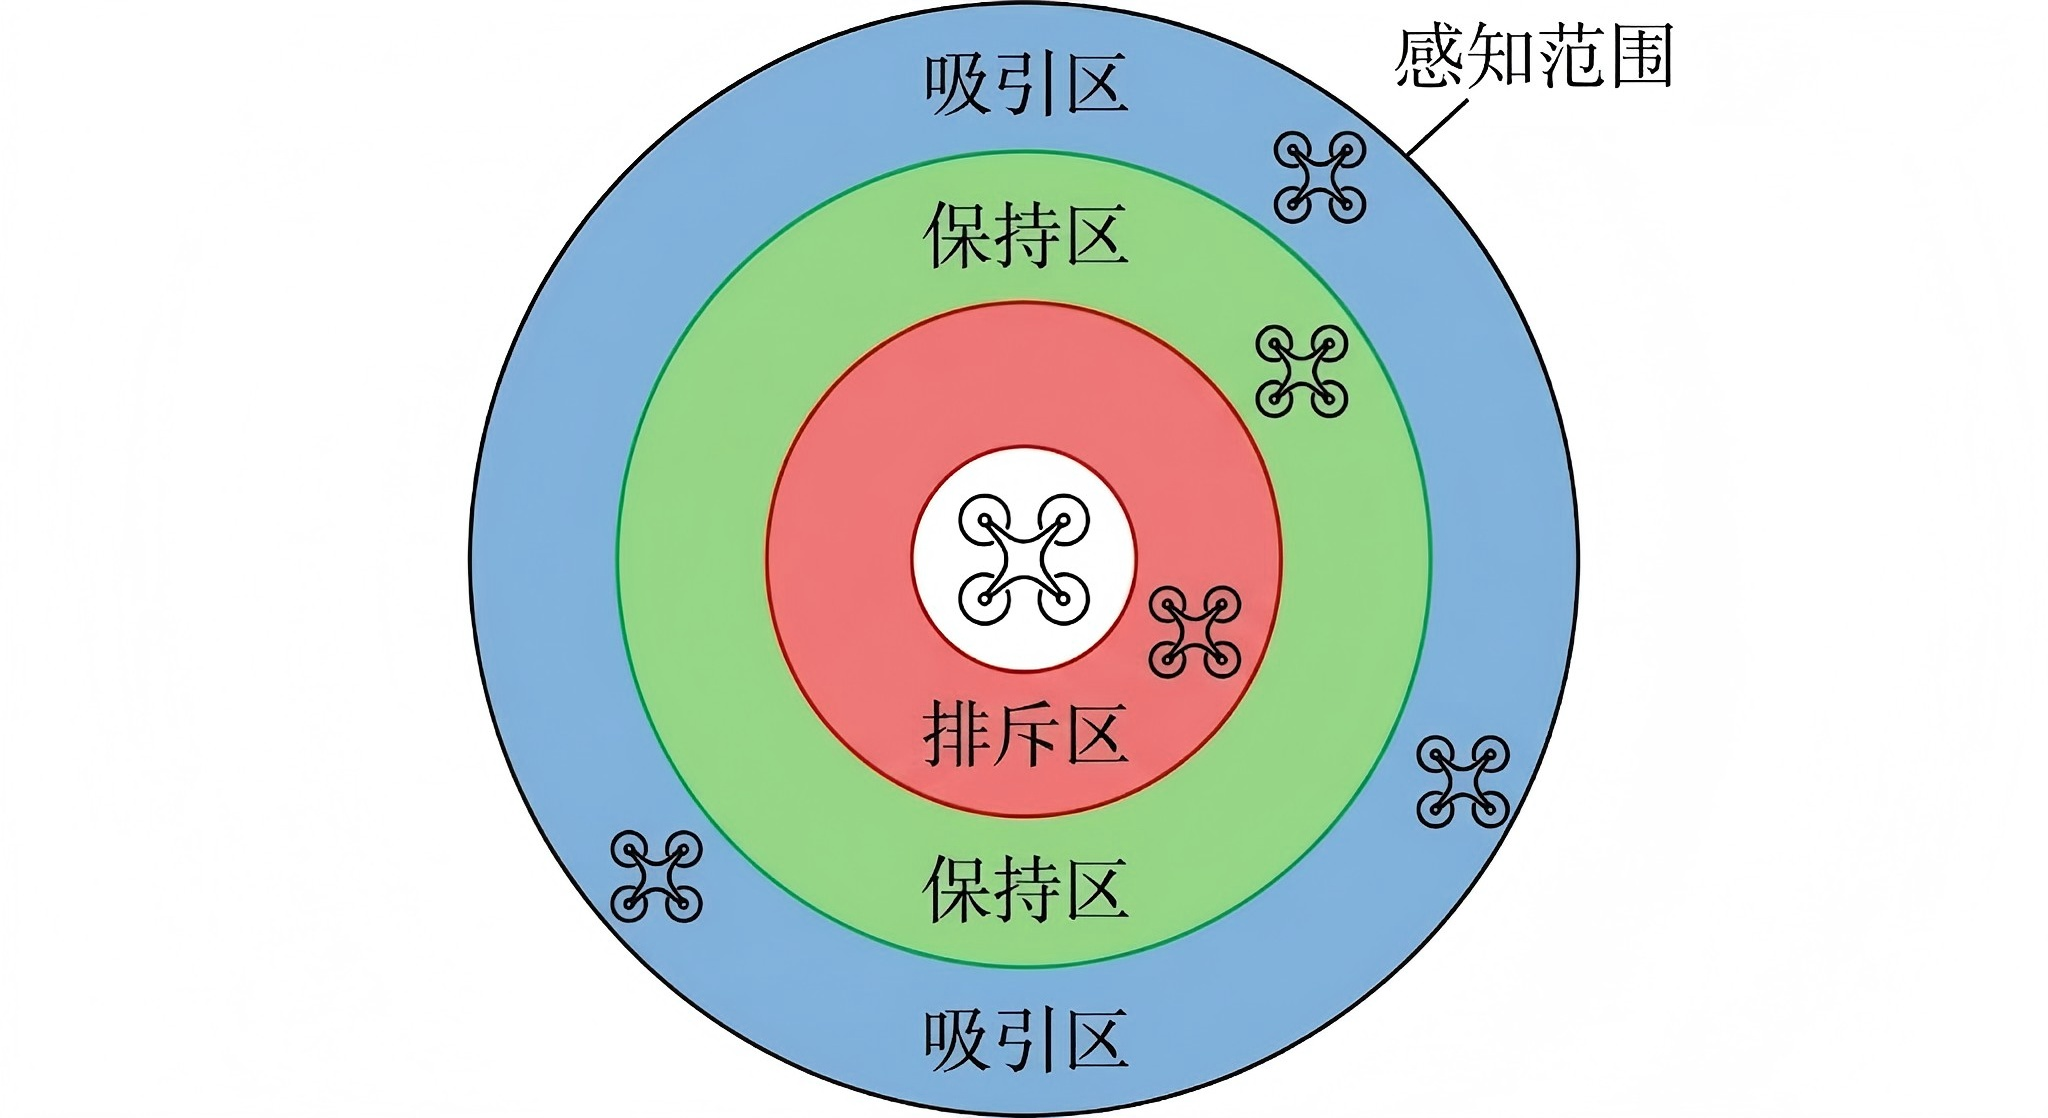
\includegraphics[height=5cm]{images/1-5}
	\caption{基于势场的编队控制方法}
	\label{基于势场的编队控制方法}
	%\vspace{-30pt}
\end{figure}

基于行为的编队控制方法的基本思想是定义无人机集群形成编队所需的几种基本控制行为，如机间避碰、自主避障、目标获取、队形保持等，通过距离、视觉、速度等传感器采集无人机集群状态信息，依据状态信息对各基本控制行为进行加权求和，即对每个基本控制行为分别求出控制量，进而对这些控制量做加权平均，求得综合控制指令，各无人机执行机构按照综合控制指令执行各个基本控制行为，从而实现无人机集群编队，如图\ref{基于行为的编队控制方法}所示。针对多任务下无人机集群形态转换僵化、难以在有序与无序相间灵活切换的问题，文献\parencite{XDFJ202501001}提出引入向心或离心对偶力构建“突变”规则，建立四规则相变模型。该方法可实现集群在一致性有序相与不一致性无序相间的高效转换，经优化后有序相形成周期缩短。此外，文献\parencite{1025813351.nh}针对密集障碍环境中定形编队易因避障冲突而失稳的问题，提出自组织编队模型，融合基于拉普拉斯矩阵的编队规则、新避障规则与约束协调机制。该方法使集群在避障时弹性形变、过后快速恢复队形，实现了安全、有序的定形编队飞行，并通过实物验证。文献\parencite{KZLY201510004}针对多无人机编队在复杂长机机动下难以保持稳定队形的问题，提出一种基于鸽群层级行为机制的编队控制方法，该方法通过有向图建模鸽群特有的上下级领导拓扑，并结合人工势场描述领导作用，使僚机仅依赖局部上级信息即可在长机剧烈机动时仍能自主维持“人”字形编队。文献\parencite{BJHK202102025}针对无人机集群通信负载大、应激响应精度低的问题，受寒鸦配对飞行行为启发，提出一种配对交互编队控制模型，该模型通过让部分无人机一对一配对，减少每机平均邻居数以降低通信量，并利用配对个体间的强耦合提升集群对外部刺激的响应精度与一致性。

\begin{figure}[H]
	\centering
	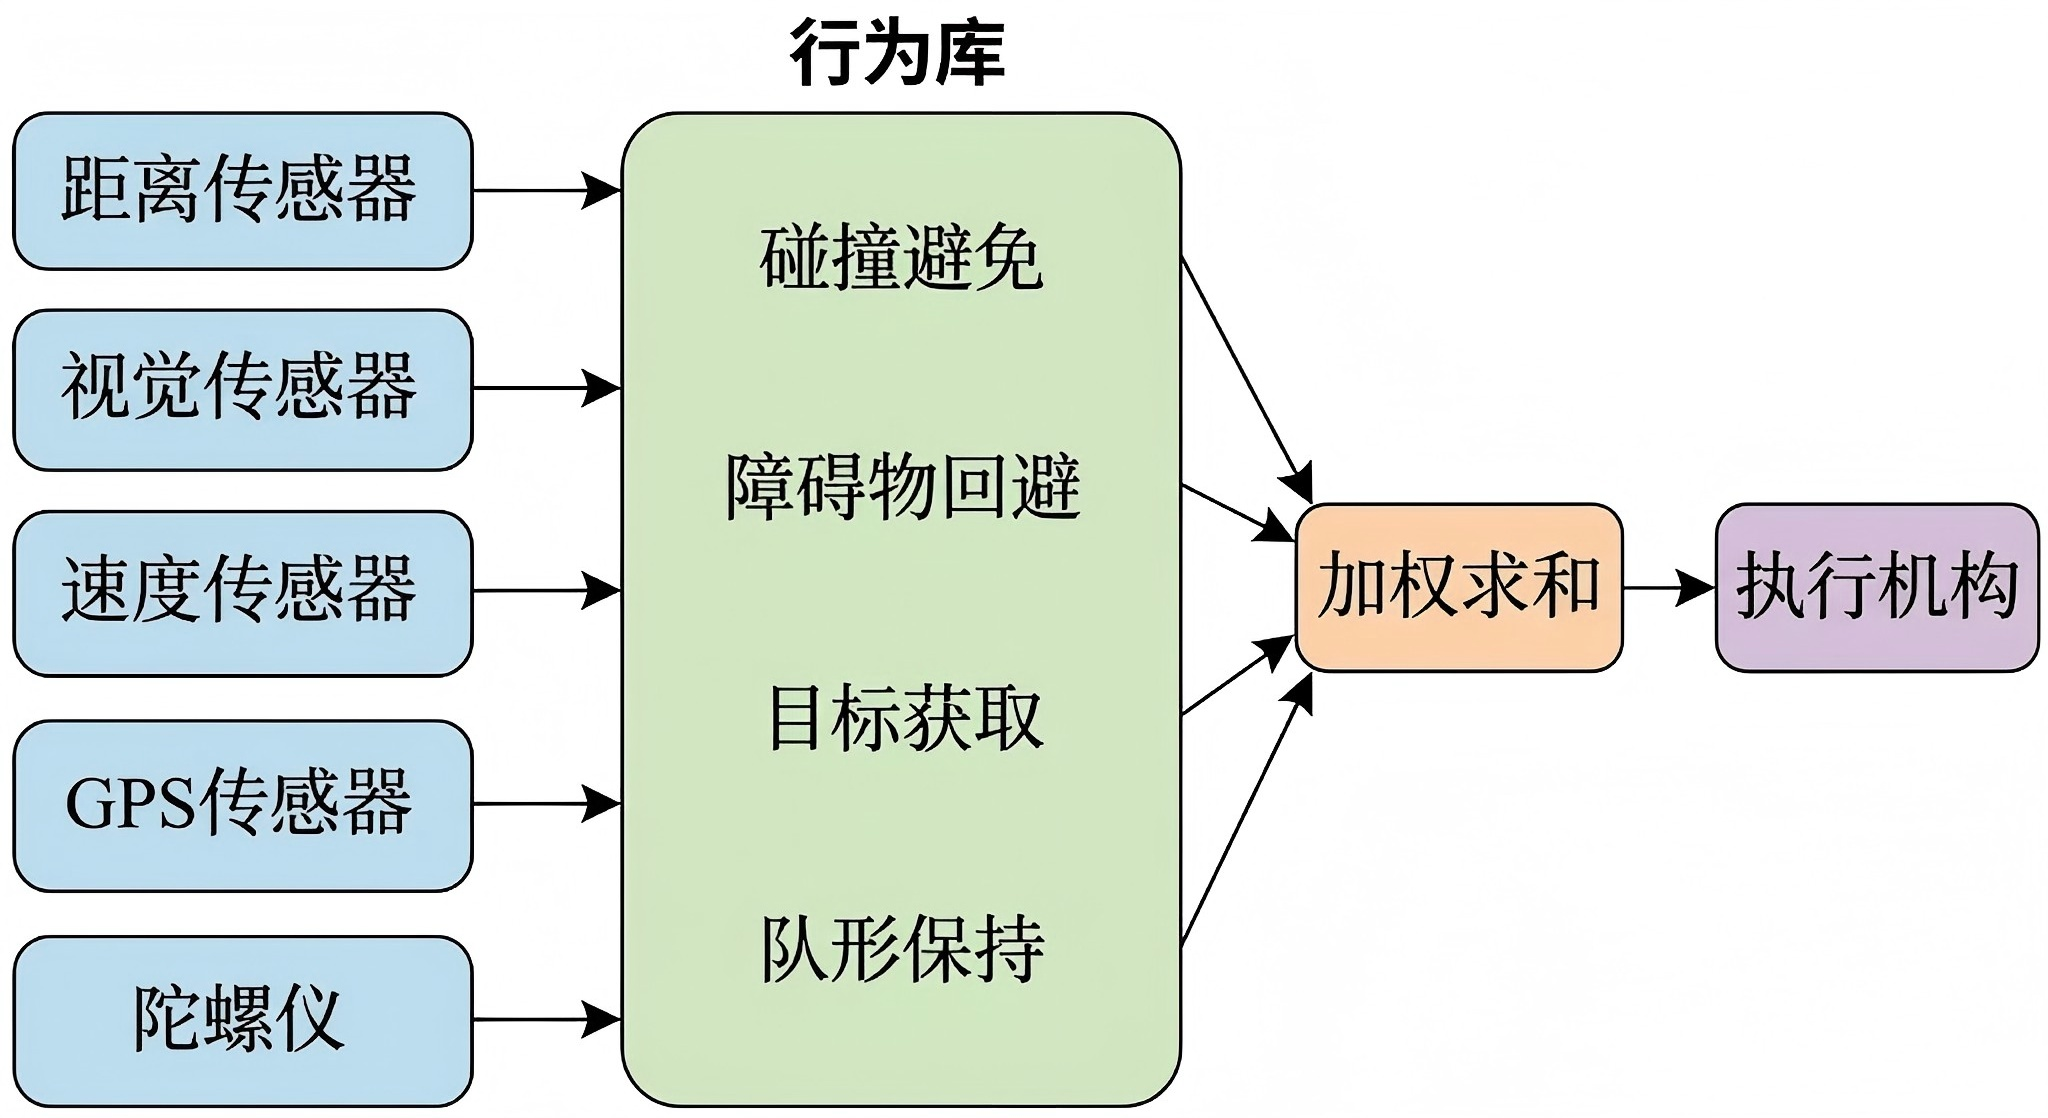
\includegraphics[height=5cm, keepaspectratio]{images/1-6}
	\caption{基于行为的编队控制方法}
	\label{基于行为的编队控制方法}
	%\vspace{-30pt}
\end{figure}

基于一致性理论的控制方法是无人机在基于分布式的网络中，利用与之通信的相邻无人机状态信息来综合更新自身状态，最终使集群内所有无人机的状态达到一致，从而实现无人机集群编队\cite{HKBQ202205007}。如图\ref{基于一致性理论的控制方法}所示。针对多无人机在一致性编队飞行中易发生碰撞的问题，文献\parencite{6858777}提出一种分层控制策略,该策略在水平面采用四阶一致性协议实现编队，在垂直方向叠加基于人工势场的避碰力，并通过Lyapunov分析证明了即使两者同时作用，系统仍能收敛到期望队形。文献\parencite{1024717699.nh}针对传统一致性方法收敛速度慢、人工势场法存在局部极小值等问题，提出一种融合改进有限时间一致性与优化人工势场的编队避障方法。通过引入路径分段和随机扰动，实现了编队在三维空间中快速成形、有效避障并顺利抵达目标。此外，文献\parencite{6798711}针对无人机集群在切换通信拓扑下难以实现时变编队与轨迹跟踪的问题，提出一种基于一致性理论的分布式编队控制器，将编队问题转化为闭环系统稳定性问题，并通过构造公共Lyapunov函数，给出了在任意切换信号下系统稳定的充分条件，有效提升了编队控制的鲁棒性与适应性。为进一步提升领航-跟随架构下的协同性能，文献\parencite{YANG2025592} 从一致性理论出发，提出一种基于位置一致性的分布式领航-跟随编队控制策略，通过引入虚拟领航者并设计新型一致性协议，有效实现了多无人机系统在动态环境下的高精度协同跟踪与稳定编队，确保状态误差全局渐近收敛。值得关注的是，文献\parencite{TANG2026103722} 进一步将一致性思想与智能学习机制相结合，提出一种基于一致性学习的分层编队控制方法，上层利用一致性协议生成协同参考轨迹，下层融合滑模自适应控制与神经网络协同学习机制，实时补偿模型不确定性与外部扰动，显著增强了多无人机系统在复杂动态环境中的轨迹跟踪精度与整体鲁棒性。而在容错一致性控制研究中，文献\parencite {LIU2025112440} 针对飞翼无人机集群存在的非一致未知方向故障与外部扰动问题，设计切换函数基最优主动容错二分一致性控制策略，融合强化学习与饱和函数优化系统暂态性能，有效抑制故障冲击与状态抖振，实现了集群姿态的二分一致性控制并提升了系统鲁棒性。

\begin{figure}[H]
	\centering
	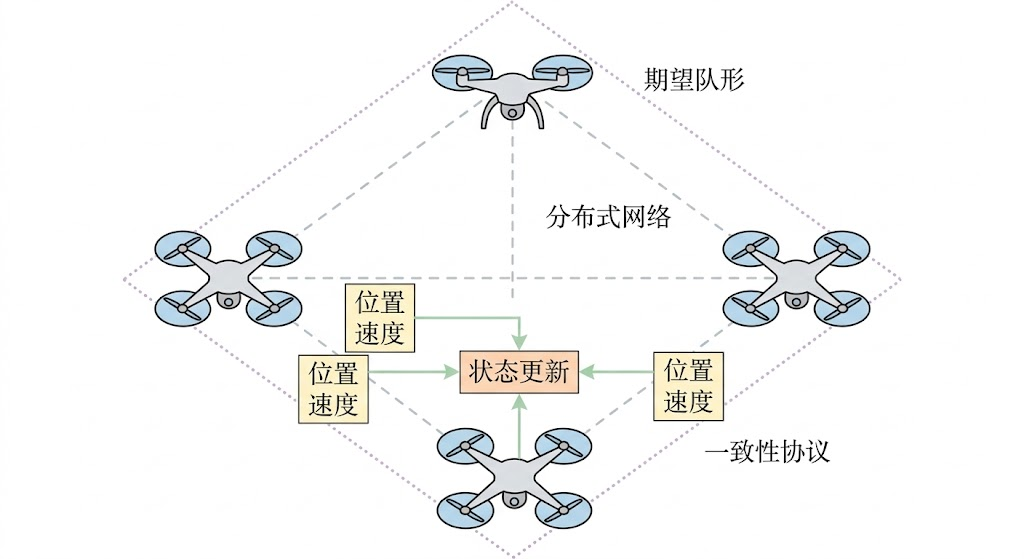
\includegraphics[height=5cm, keepaspectratio]{images/1-7}
	\caption{基于一致性理论的控制方法}
	\label{基于一致性理论的控制方法}
	%\vspace{-30pt}
\end{figure}

\subsection{研究现状总结}
综上所述，无人机集群编队控制技术已取得显著进展，分布式控制架构因其固有的鲁棒性与可扩展性，已成为应对复杂任务场景的主流范式。然而，现有研究大多建立在无人机能够获取全维的位置状态信息，这一情况在GNSS拒止、通信受限或传感器能力异构等真实复杂环境中往往难以成立。

当前研究在处理非全维位置量测这一现实约束时，仍存在明显不足。一方面，许多先进的编队控制算法高度依赖全局或完整的局部位置信息，当部分维度的状态缺失时，其性能会急剧下降甚至失效。另一方面，虽然分布式架构降低了对中心节点的依赖，但若个体无法有效估计自身或邻居的全维状态，协同控制的基础便不复存在。如何在仅有部分绝对位置和相对距离量测的条件下，实现整个集群状态的有效感知与稳定协同，是当前研究亟待突破的关键瓶颈。

针对此问题，本课题将研究重心聚焦于非全维量测条件下的分布式编队控制。具体而言，本文拟从系统可观测性分析、分布式状态观测器设计和鲁棒协同控制器构建三个层面展开系统性研究，为无人机集群在真实受限环境中的可靠、高效运行提供一套完整的理论方法与技术方案。
\section{研究内容与章节安排}

\subsection{研究内容}
\textbf{1）无人机集群异构传感模型建立：}
考虑四旋翼无人机刚体动力学欠驱动系统特征，将底层姿态控制与顶层编队协同解耦，采用二阶积分器模型简化集群运动描述，构建适用于协同控制的质点动力学模型。结合图论数学工具，精准表征无人机集群节点间的通讯拓扑关系与刚性编队约束，明确编队框架的无穷小刚性与一阶刚性判断条件。系统研究GNSS拒止环境下异构传感器的量测特性，区分不同量测条件无人机的量测机制并建立专属量测方程。最终形成 “刚体动力学模型+分层网络架构+异构量测方程” 的完整模型体系，为后续可观测性分析与控制算法设计提供坚实支撑。

\textbf{2）编队系统可观测性分析与传感器配置：}
基于刚性理论深入研究异构传感配置下编队系统的可观测性问题，明确 “部分位置+相对距离” 量测模式下的 “弱可观测性” 定义与判定准则。推导保证系统弱可观测的要求，量化锚点布局对系统可观性的影响权重。
研究基于矩阵QR分解的传感器配置策略，通过对可观测性矩阵进行QR分解，建立锚点数量、空间位置与系统可观性之间的量化关系。设计锚点优化部署算法，确保在传感器成本等约束下，通过最少锚点配置实现整个集群系统的弱可观测性。

\textbf{3）基于异构传感融合的分布式状态观测器设计：}
针对异构传感模型的量测特性，设计分布式全维状态观测器，实现所有无人机位置与速度的完整估计。构建融合机间距离量测与邻居节点估计信息的分布式更新机制，设计状态估计算法，使得跟随无人机能够通过与相邻节点的局部信息交互，逐步修正自身状态估计值，突破仅依赖相对距离无法估计全维状态的技术瓶颈。

\textbf{4）动态轨迹跟踪鲁棒协同控制器设计：}
基于状态观测器输出的全维状态估计值，设计适配动态轨迹跟踪的鲁棒协同控制器。控制器采用 “位置反馈+梯度控制” 的复合控制结构：位置反馈项基于无人机当前估计状态与期望轨迹的偏差设计，确保轨迹跟踪的精准性；梯度控制项基于机间距离约束设计，引入机间最小安全距离与最大通信距离阈值，通过势场函数或梯度下降法生成避碰与队形保持指令，实现编队稳定与机间碰撞规避的协同优化。
通过观测器与控制器的闭环耦合设计，实现状态估计误差与编队跟踪误差的联合收敛，增强系统在复杂扰动环境下的整体性能。

\textbf{5）协同定位与编队控制仿真验证:}
在MATLAB/Gazebo仿真环境中构建海洋GNSS拒止等典型复杂场景，搭建包含锚点无人机与跟随无人机的异构集群仿真系统。设置动态轨迹跟踪任务，引入量测噪声等扰动因素，验证所设计的分布式观测器的状态估计收敛性；设计融合位置估计与机间距离约束的鲁棒协同控制器，确保编队稳定保持，并通过误差曲线分析与轨迹可视化，评估控制方法的鲁棒性与动态适应性。
\subsection{章节安排}
本文围绕大规模无人机集群在复杂环境下的分布式编队控制问题展开研究，聚焦于系统可观测性、状态观测和鲁棒控制三个方面，整体研究路径按照无人机集群建模、异构传感器配置、编队状态观测、编队跟踪控制以及仿真验证的逻辑展开。具体内容的组织架构如图\ref{论文组织架构}所示。

\begin{figure}[H]
	\centering
	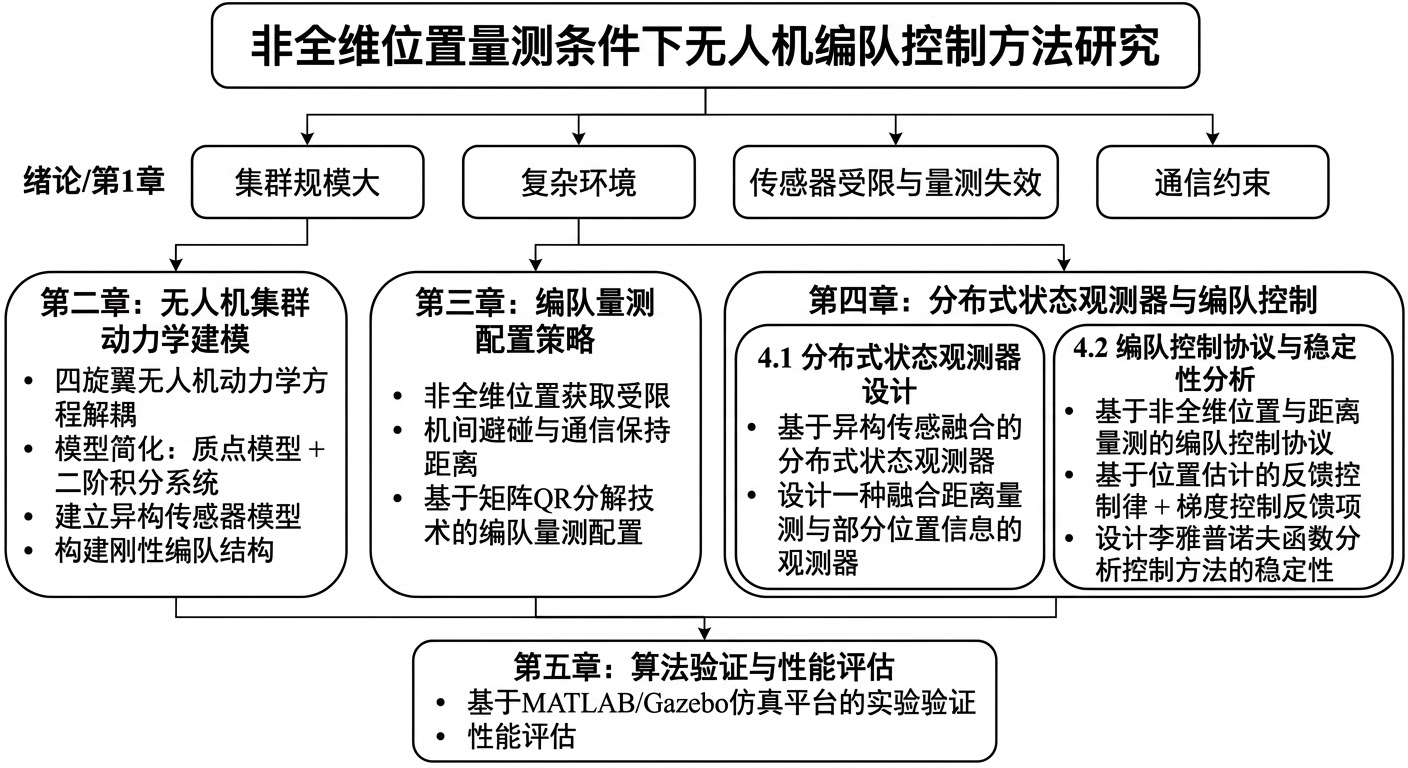
\includegraphics[width=1\linewidth]{images/1-8}
	\caption{论文组织架构}
	\label{论文组织架构}
	%\vspace{-30pt}
\end{figure}

本文共分为五章：第一章为绪论，阐述研究背景、意义及国内外现状，并明确本文的研究内容与创新点。第二章建立适用于协同控制的无人机集群异构传感模型，为后续分析奠定基础。第三章聚焦于编队系统的可观测性，基于刚性理论分析并提出最优的锚点传感器配置策略。第四章是核心算法设计，首先构建分布式全维状态观测器以解决非全维量测问题，进而设计动态轨迹跟踪的鲁棒协同控制器。第五章在MATLAB/Gazebo仿真环境中，对所提出的观测与控制方法进行系统性验证，评估其在复杂场景下的有效性与鲁棒性。

\section{主要贡献及创新点}
\textbf{1）明确异构传感下 “弱可观测性” 理论边界：}
基于刚性理论提出非全维量测条件下的弱可观性判据，保证系统可观测的最小锚点数量与空间配置要求，为传感器部署提供清晰的理论依据。

\textbf{2）轻量化分布式状态观测器设计：}
采用一阶泰勒展开对非线性距离量测进行线性化处理，在保证精度的同时降低计算复杂度；构建融合非全维局部量测与邻居估计信息的分布式更新机制，突破仅依赖相对距离无法估计全维状态的技术瓶颈。

\textbf{3）动态适配的鲁棒协同控制框架：}
控制器设计兼容时变期望轨迹，突破传统静态编队保持的局限；实现集群系统的局部稳定收敛，增强动态场景下的编队稳定性与避碰安全性。

\textbf{4）高保真仿真验证体系：}
搭建异构集群仿真平台，模拟海洋GNSS拒止等真实场景，系统评估量测噪声、通信延迟等扰动下的性能表现，为工程落地提供数据支撑。
